\pagestyle{empty}
\tikzstyle{every picture}+=[remember picture]
\everymath{\displaystyle}

\begin{figure}[!ht]

\centering
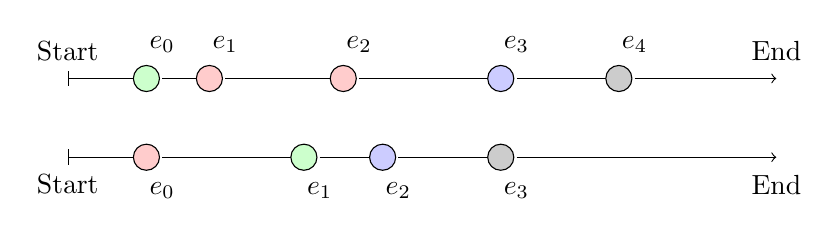
\begin{tikzpicture}

% FIRST TIMELINE

\draw[|-] (1,0) node[below=1mm]{Start} -- (2,0) node{\tikz[baseline]{
	\node[fill=red!20,draw,circle] (e0){};
}
};
\draw[-] (2.2,0) node[below=2mm]{$e_0$} -- (4,0) node{\tikz[baseline]{
	\node[fill=green!20,draw,circle] (e1){};
}
};
\draw[-] (4.2,0) node[below=2mm]{$e_1$} -- (5,0) node{\tikz[baseline]{
	\node[fill=blue!20,draw,circle] (e2){};
}
};
\draw[-] (5.2,0) node[below=2mm]{$e_2$} -- (6.5,0) node{\tikz[baseline]{
	\node[fill=black!20,draw,circle] (e3){};
}
};
\draw[->] (6.7,0) node[below=2mm]{$e_3$} -- (10,0) node[below=1mm]{End};

% SECOND TIMELINE

\draw[|-] (1,1) node[above=1mm]{Start} -- (2,1) node{\tikz[baseline]{
	\node[fill=green!20,draw,circle] (f0){};
}
};
\draw[-] (2.2,1) node[above=2mm]{$e_0$} -- (2.8,1) node{\tikz[baseline]{
	\node[fill=red!20,draw,circle] (f1){};
}
};
\draw[-] (3,1) node[above=2mm]{$e_1$} -- (4.5,1) node{\tikz[baseline]{
	\node[fill=red!20,draw,circle] (f2){};
}
};
\draw[-] (4.7,1) node[above=2mm]{$e_2$} -- (6.5,1) node{\tikz[baseline]{
	\node[fill=blue!20,draw,circle] (f3){};
}
};
\draw[-] (6.7,1) node[above=2mm]{$e_3$} -- (8,1) node{\tikz[baseline]{
	\node[fill=black!20,draw,circle] (f4){};
}
};
\draw[->] (8.2,1) node[above=2mm]{$e_4$} -- (10,1) node[above=1mm]{End};

\end{tikzpicture}

% Now it's time to draw some edges between the global nodes. Note that we
% have to apply the 'overlay' style.
\begin{tikzpicture}[overlay]
        \path[->] (f0) edge [out=-90, in=135] (e1);
        \path[->] (e2) edge [out=45, in=-135] (f3);
        \path[->] (e3) edge [out=45, in=-135] (f4);
\end{tikzpicture}

  \caption{An example of a simulation. Red circles are peers' internal events.}
\end{figure}
